\section{In-distribution results}
\label{sec:exp}

\subsection{Training dynamics}
Validation tracks training closely for both models (\cref{fig:curves}); there is no overfitting gap,
and early stopping halts the teacher at $71$ and the student at $34$ epochs. The distilled student's
validation accuracy converges above the teacher's, foreshadowing the result below.

\begin{figure*}[tb]
  \centering
  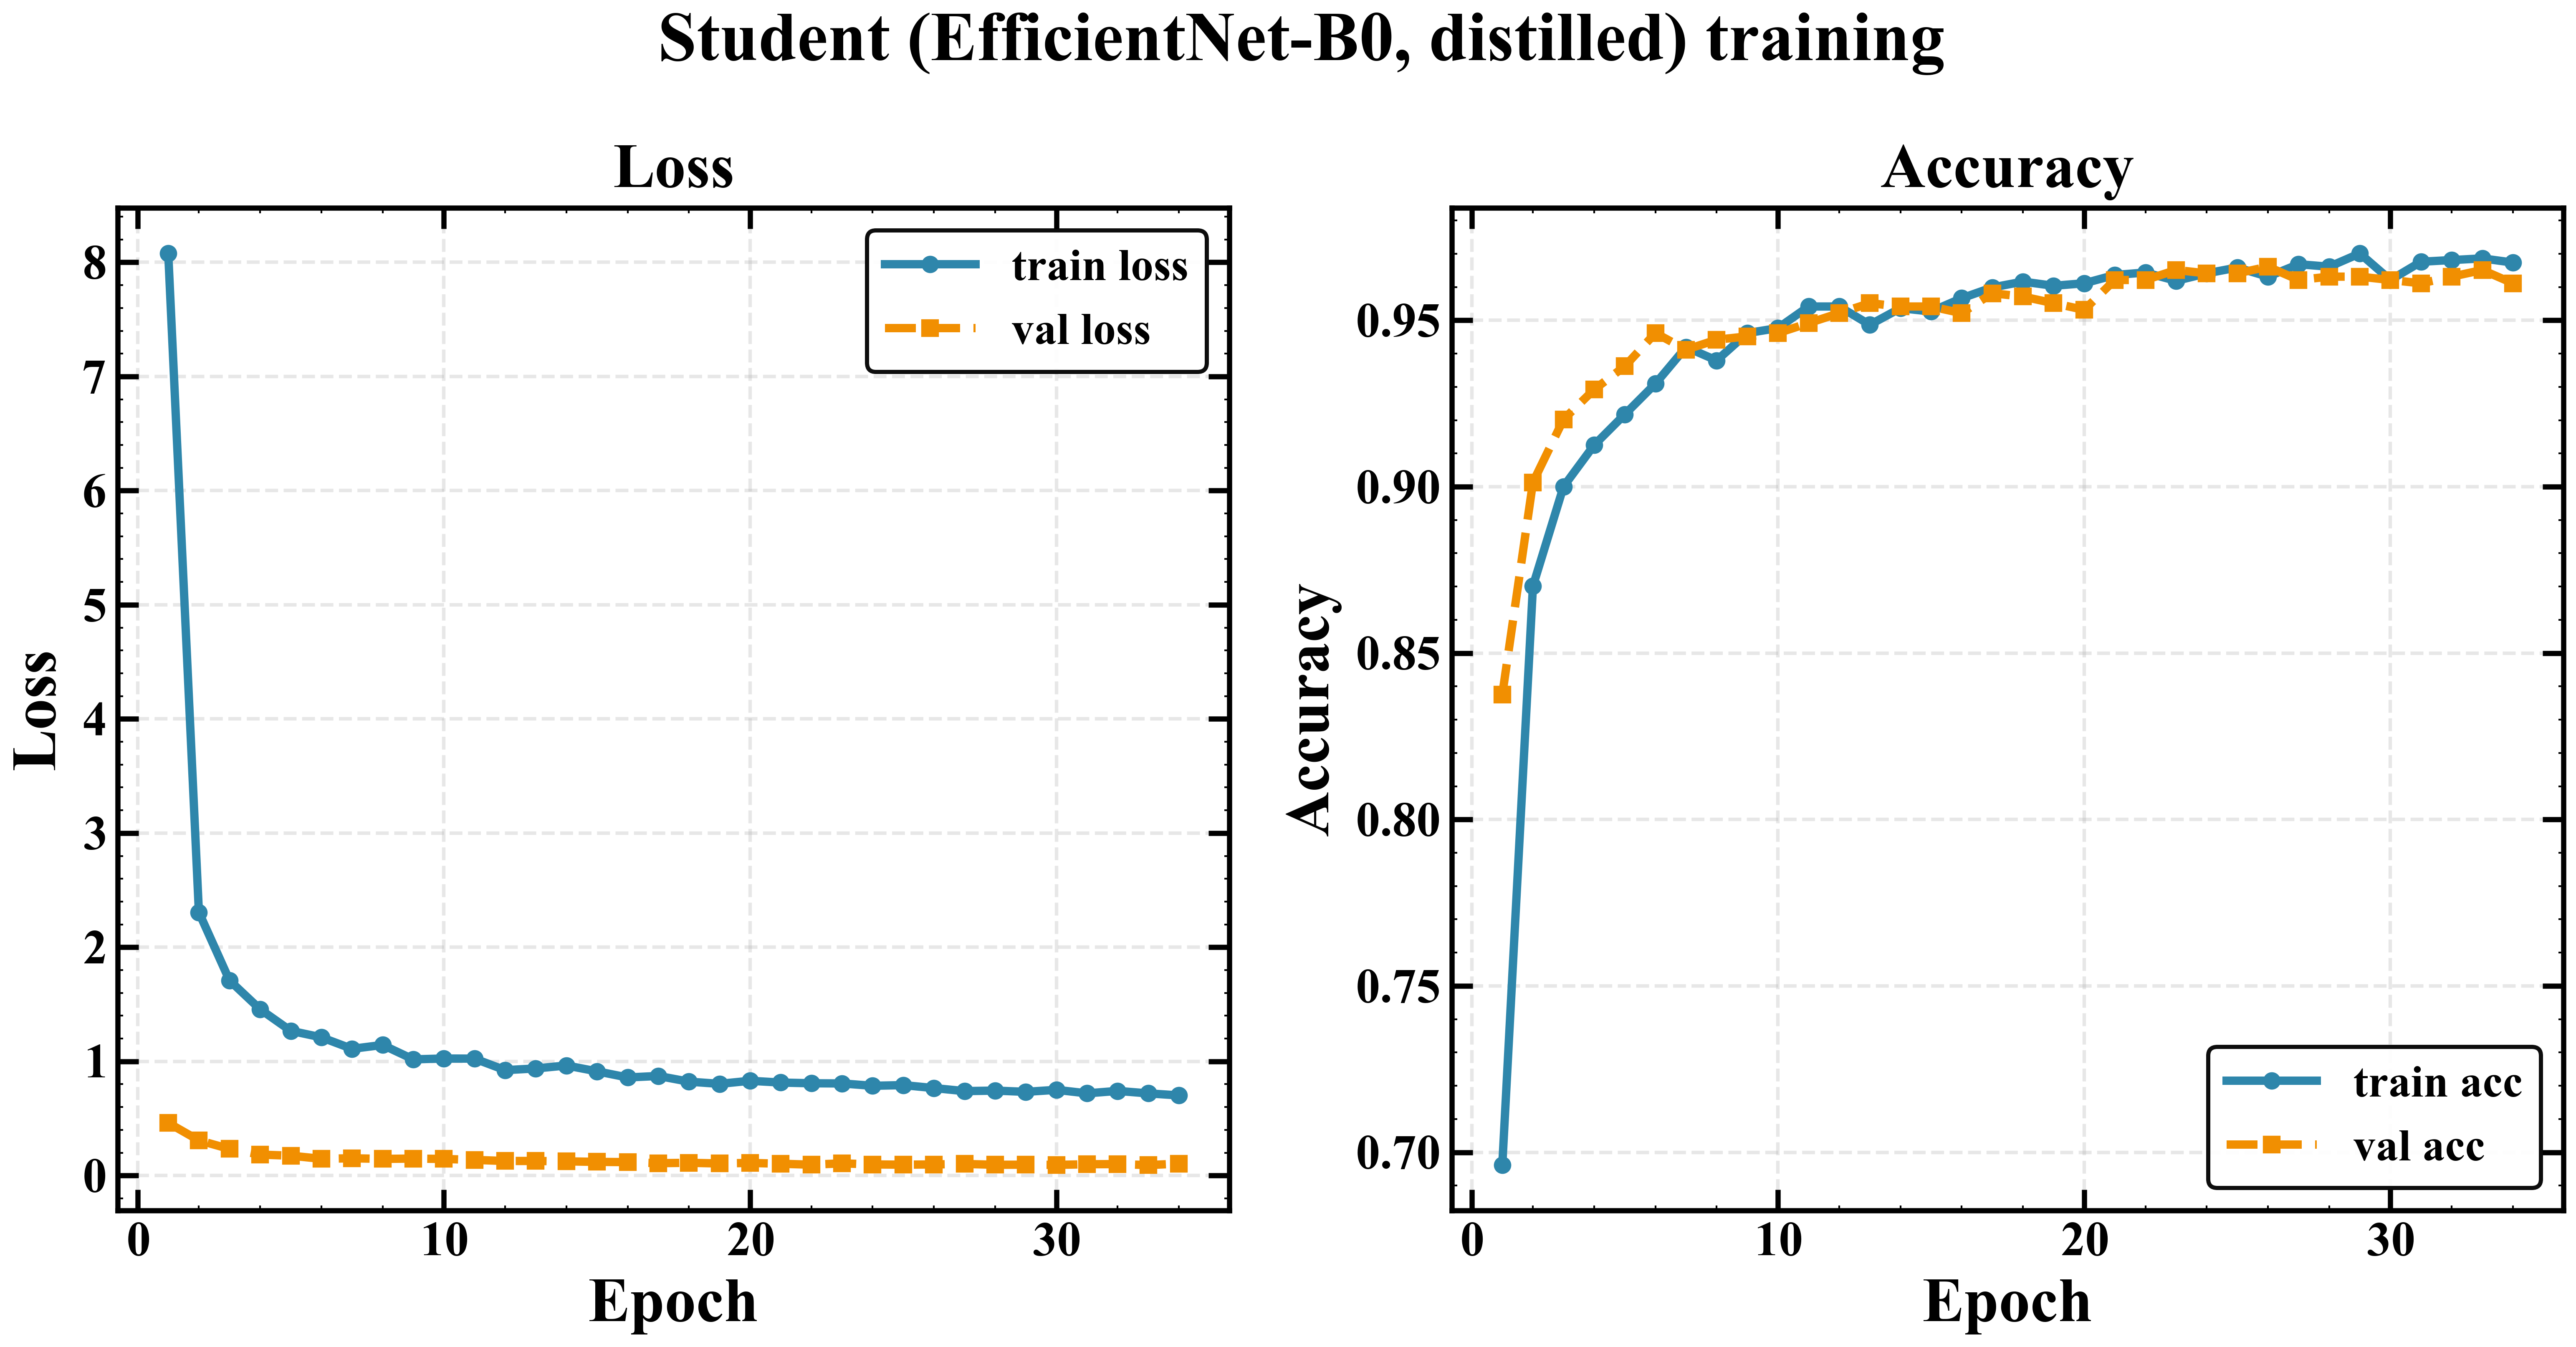
\includegraphics[width=0.49\textwidth]{student_training_curves.png}\hfill
  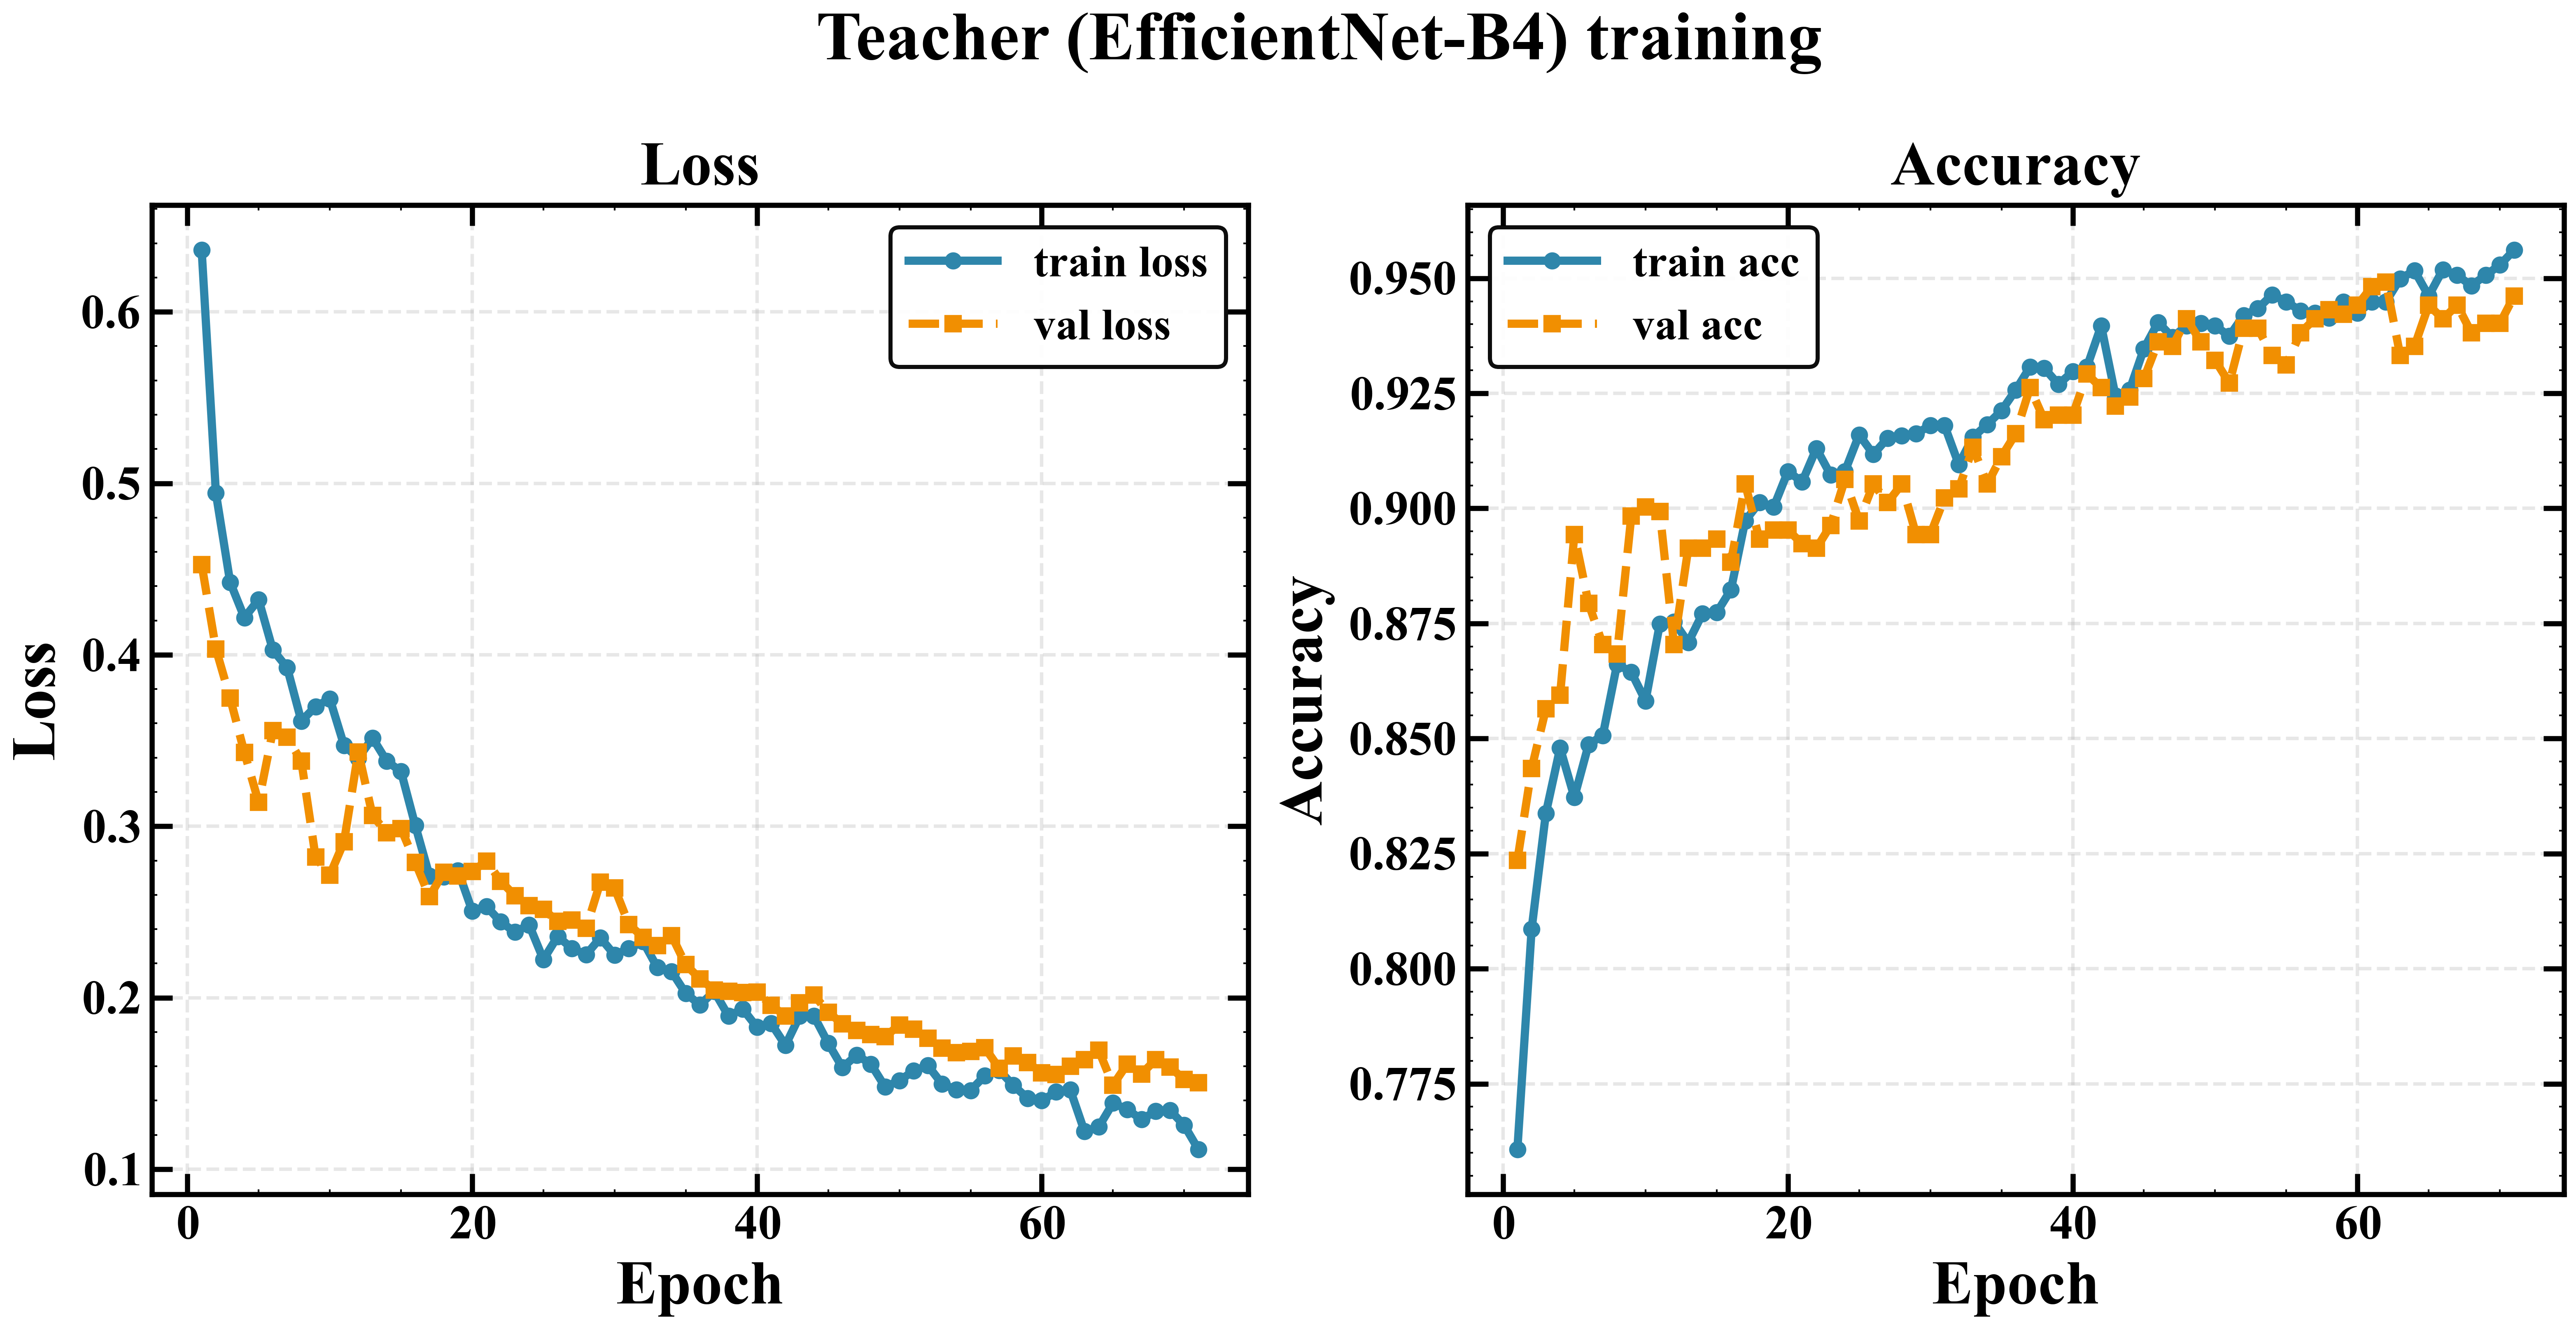
\includegraphics[width=0.49\textwidth]{teacher_training_curves.png}
  \caption{\textbf{Training dynamics.} Left: distilled B0 student ($34$ epochs). Right: B4 teacher
  (two stages, $71$ epochs). Validation tracks training in both---no overfitting.}
  \label{fig:curves}
\end{figure*}

\subsection{Classification performance (answering RQ1)}

\begin{table}[t]
\caption{\textbf{In-distribution five-class metrics.} \sipakmed\ validation, $n{=}1003$. The distilled
student surpasses its teacher on every metric and is well calibrated.}
\label{tab:indist}
\centering\small
\begin{tabular}{@{}lcc@{}}
\toprule
Metric & Teacher (B4) & \best{Student (B0)} \\
\midrule
Parameters         & 18.5\,M & \best{4.67\,M} \\
Accuracy           & 0.943 & \best{0.966} \\
Balanced accuracy  & 0.946 & \best{0.968} \\
Macro-$F_1$        & 0.945 & \best{0.967} \\
Cohen's $\kappa$   & 0.929 & \best{0.958} \\
AUROC (OvR macro)  & 0.995 & \best{0.998} \\
ECE (5-class)      & 0.013 & 0.015 \\
\bottomrule
\end{tabular}
\end{table}

\cref{tab:indist} reports the five-class metrics on the held-out \sipakmed\ validation split
($n{=}1003$). The distilled student reaches accuracy $0.966$, macro-$F_1$ $0.967$, Cohen's $\kappa$
$0.958$ and AUROC $0.998$, and \emph{exceeds the teacher on every metric} despite carrying $4\times$
fewer parameters---supporting \textbf{H1} and exposing a distillation paradox we return to in
\cref{sec:discussion}. The soft teacher targets evidently regularise the student rather than merely
compress it. Per-class (\cref{tab:perclass}, \cref{fig:cm}), the model is near-perfect on
Superficial-Intermediate and Parabasal ($F_1\,0.995/0.994$) and weakest on \emph{Koilocytotic}
($F_1\,0.919$, recall $0.873$), whose koilocytic halo overlaps morphologically with neighbouring
classes; this single class accounts for most of the in-distribution error.

\begin{table}[t]
\caption{\textbf{Per-class metrics (student).} Precision, recall and $F_1$ on the \sipakmed\
validation split. Koilocytotic is the weakest class.}
\label{tab:perclass}
\centering\small
\begin{tabular}{@{}lcccc@{}}
\toprule
Class & P & R & $F_1$ & $n$ \\
\midrule
Superficial-Intermediate & 0.990 & 1.000 & 0.995 & 191 \\
Parabasal                & 0.989 & 1.000 & 0.994 & 179 \\
Dyskeratotic             & 0.958 & 0.986 & 0.971 & 207 \\
Metaplastic              & 0.933 & 0.981 & 0.957 & 213 \\
Koilocytotic             & 0.969 & 0.873 & 0.919 & 213 \\
\bottomrule
\end{tabular}
\end{table}

\begin{figure}[t]
  \centering
  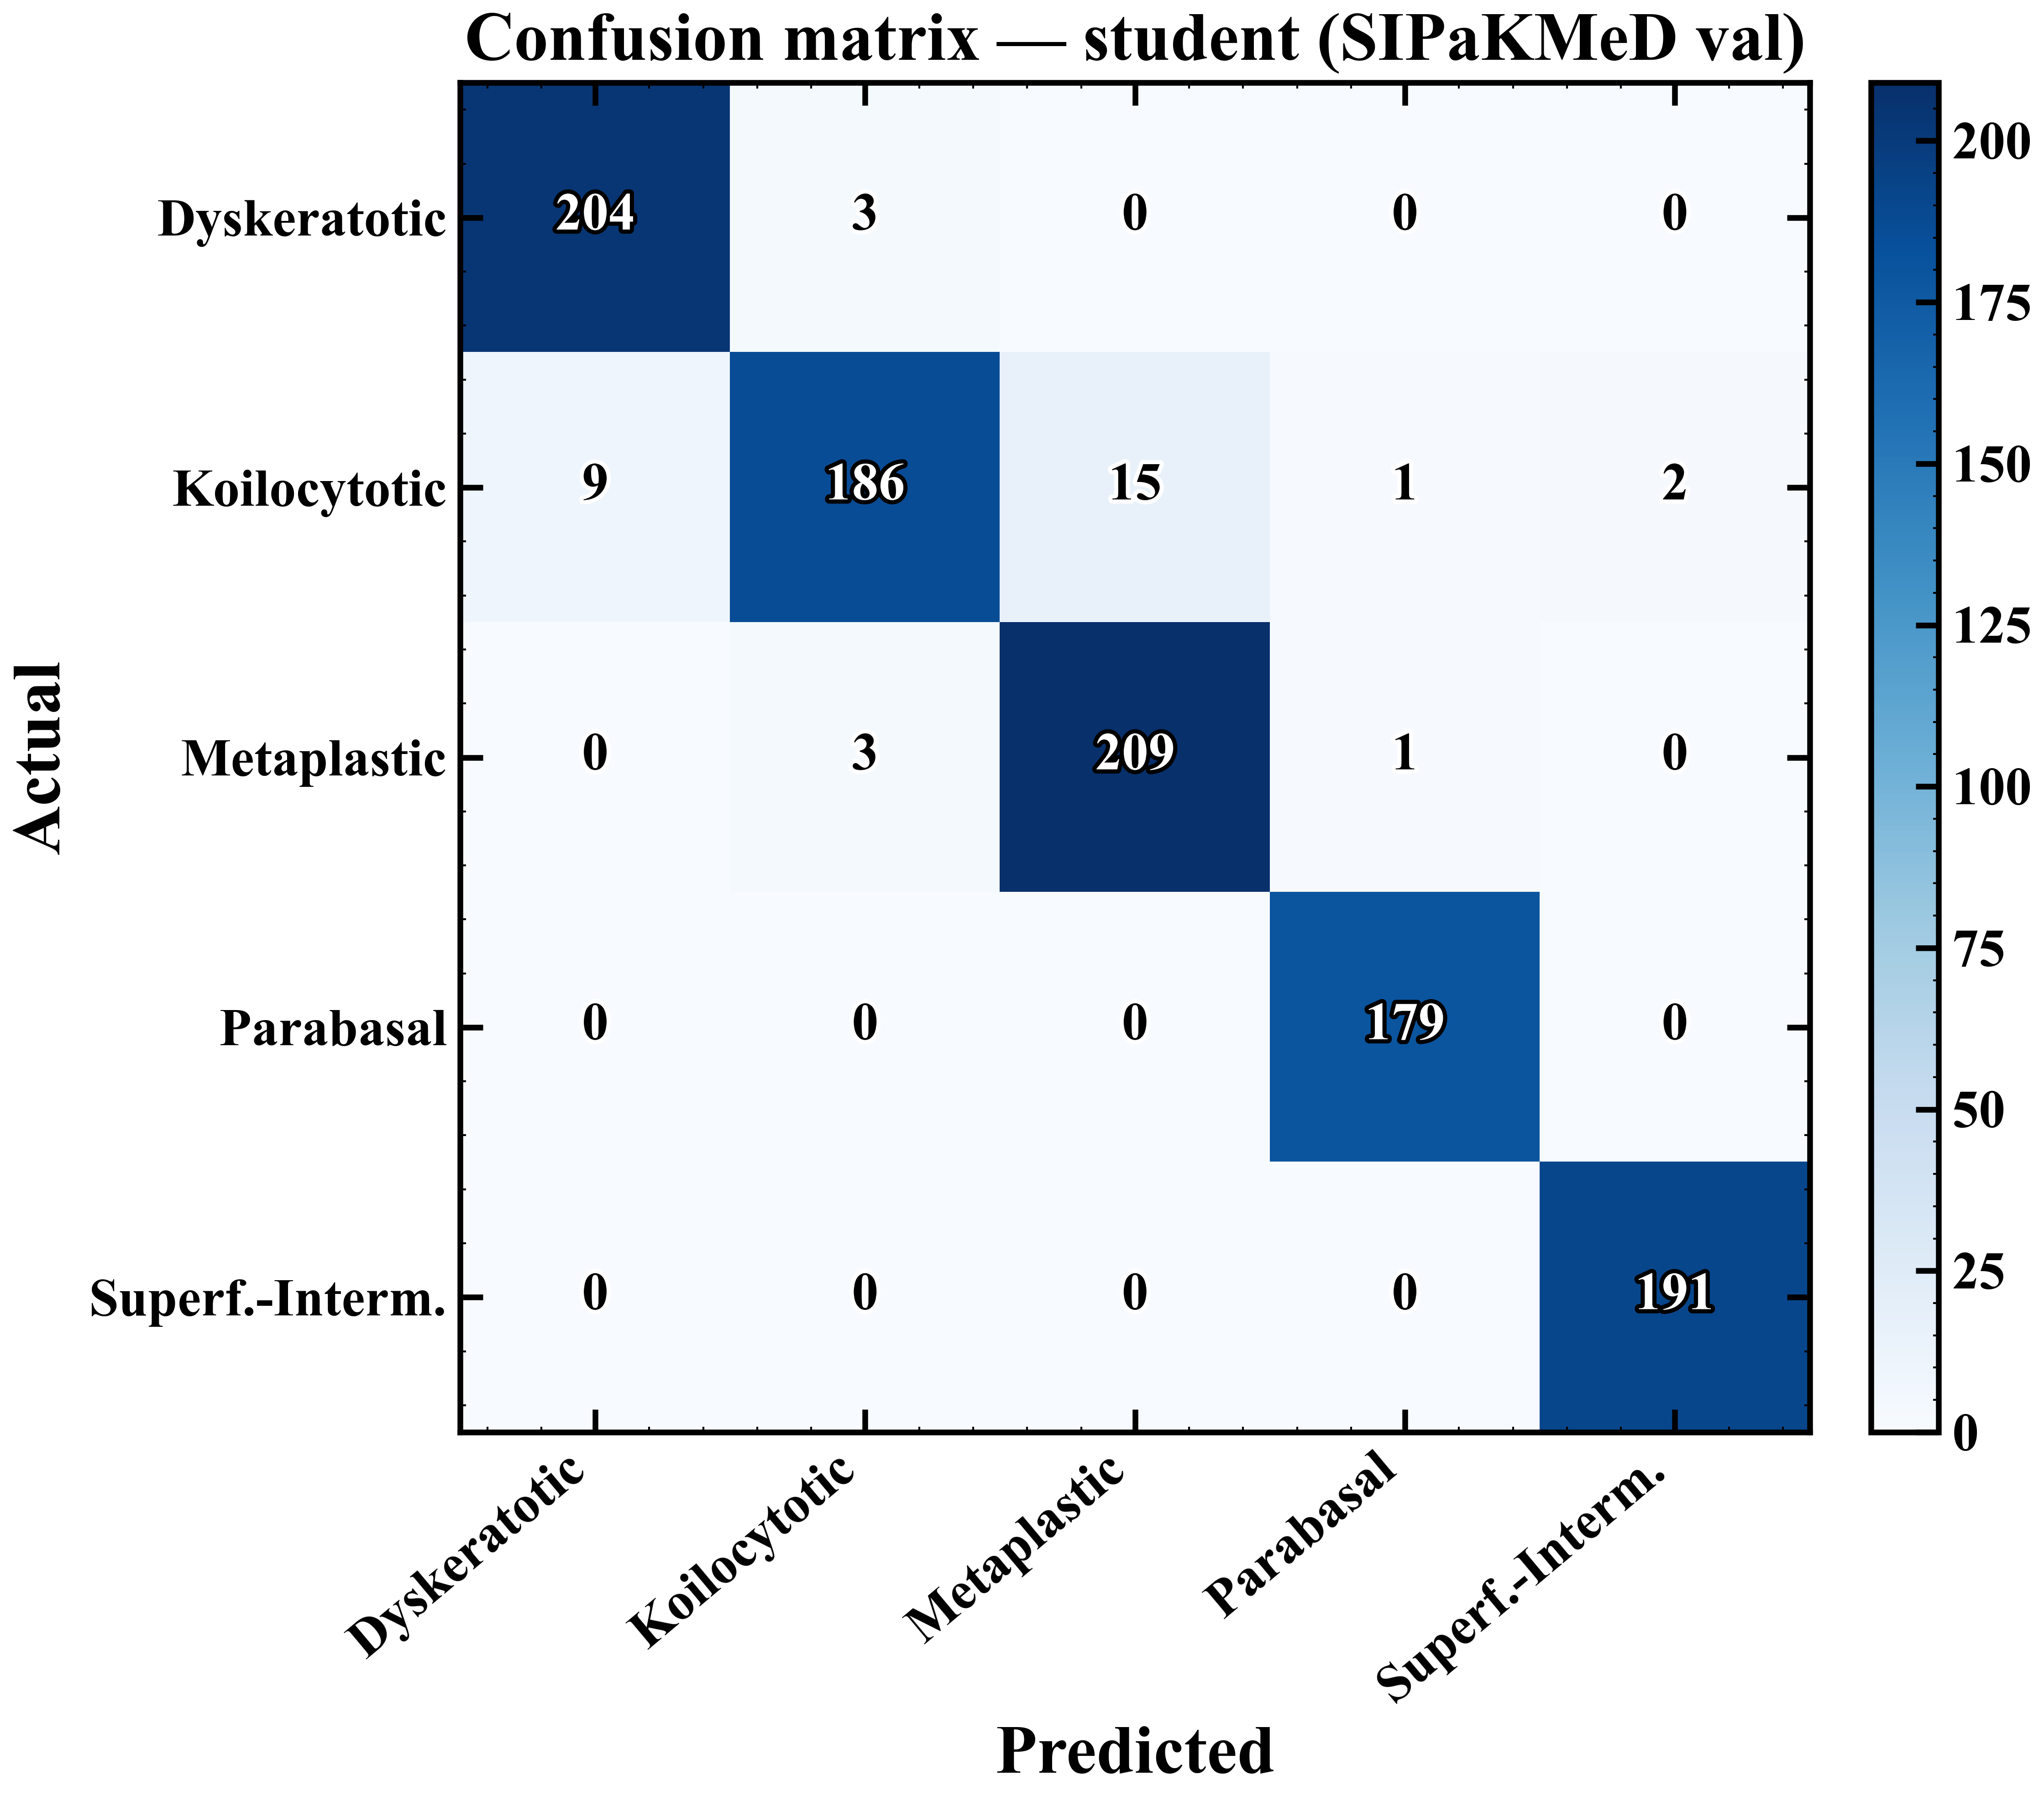
\includegraphics[width=\linewidth]{cm_student.png}
  \caption{\textbf{Five-class confusion matrix (student).} Errors concentrate on Koilocytotic.}
  \label{fig:cm}
\end{figure}

\subsection{Calibration and explainability (answering RQ4, in-distribution)}
Both models are well calibrated in-distribution: ECE $0.013$ (teacher) and $0.015$ (student) on the
five-class problem, falling to $0.008$ for the student on the binary Normal/Abnormal decision, with
reliability bins close to the identity (\cref{fig:reliability}). We carry the binary value forward as
the in-distribution calibration reference, because the cross-dataset evaluation of \cref{sec:analysis}
is binary. Grad-CAM~\cite{selvaraju2017gradcam} over the student's final convolutional block
(\cref{fig:gradcam}) localises the evidence to the nucleus and cell body for one representative
correctly-classified cell per class (confidences $0.97\!-\!1.00$). The attributions are cytologically
plausible---decisions are driven by cell structure, not background artefacts---supporting the
in-distribution half of \textbf{H4}. We stress the standard faithfulness caveat: Grad-CAM shows
\emph{where the model looked}, not that its reasoning is clinically correct. As \cref{sec:analysis}
shows, this in-distribution calibration does \emph{not} survive domain shift.

\begin{figure}[t]
  \centering
  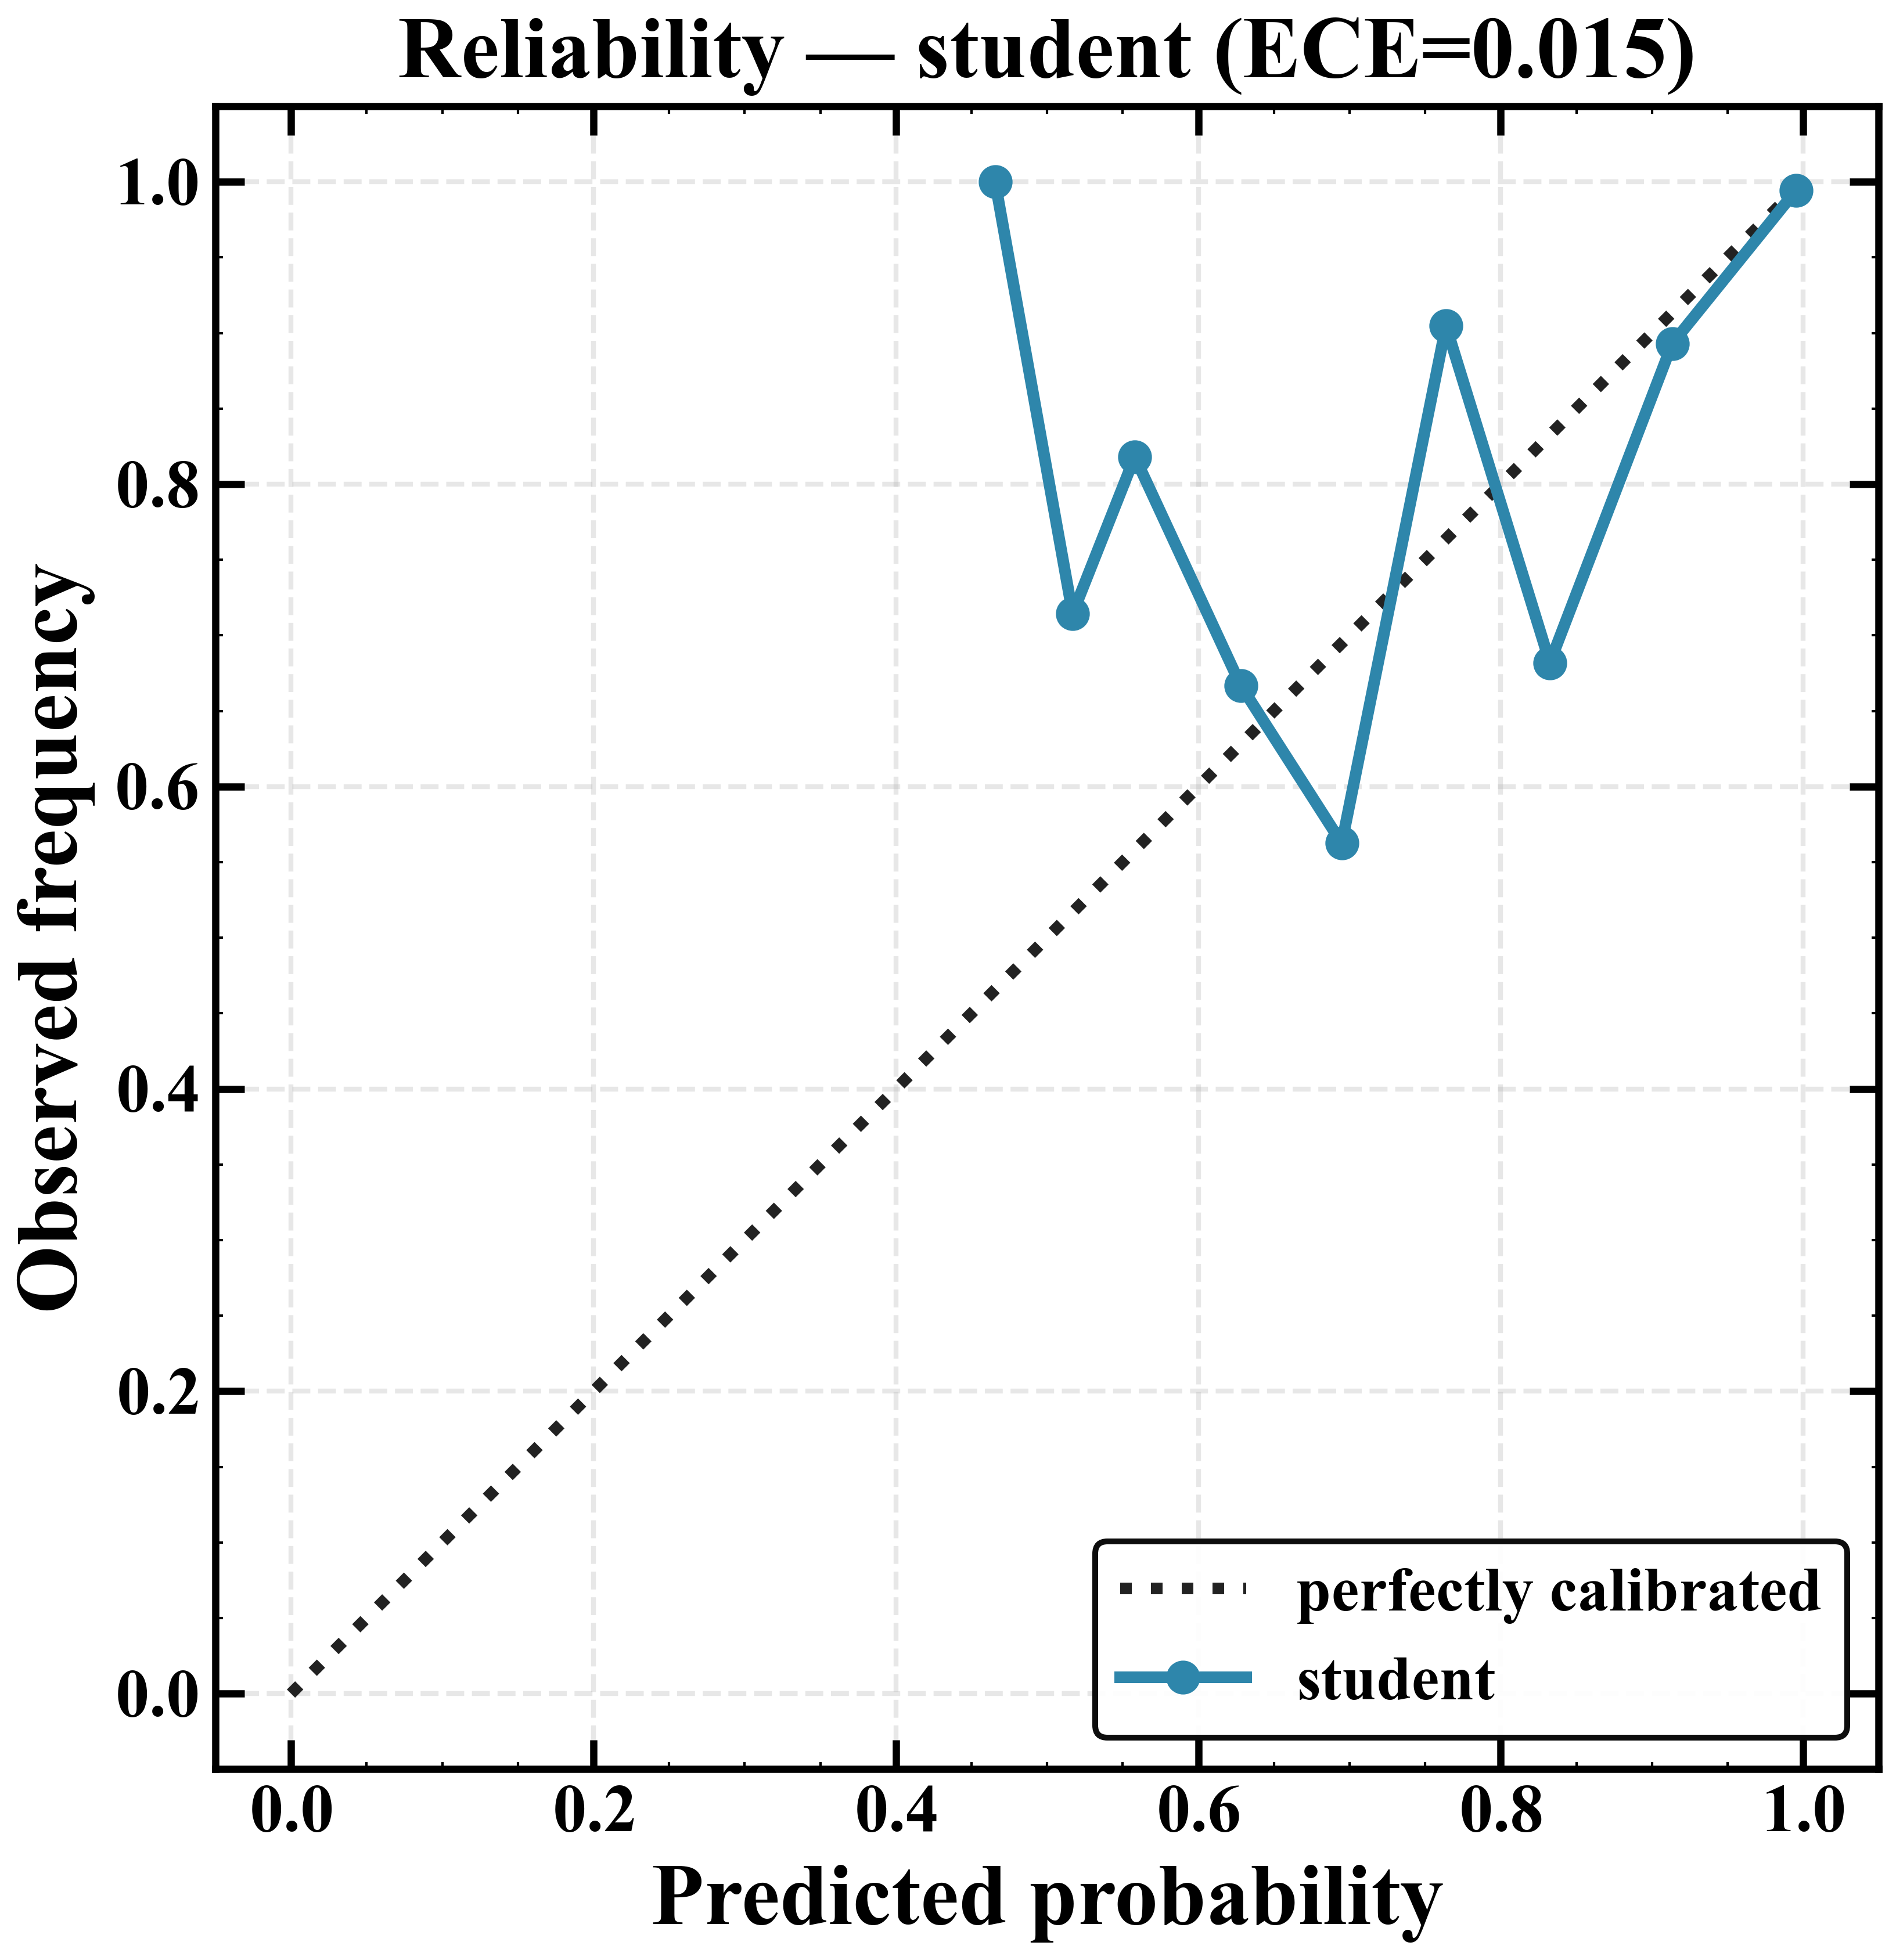
\includegraphics[width=\linewidth]{reliability_student.png}
  \caption{\textbf{Reliability diagram (student).} ECE $0.015$ (five-class): in-distribution
  confidence is well calibrated and sits close to the identity.}
  \label{fig:reliability}
\end{figure}

\begin{figure*}[tb]
  \centering
  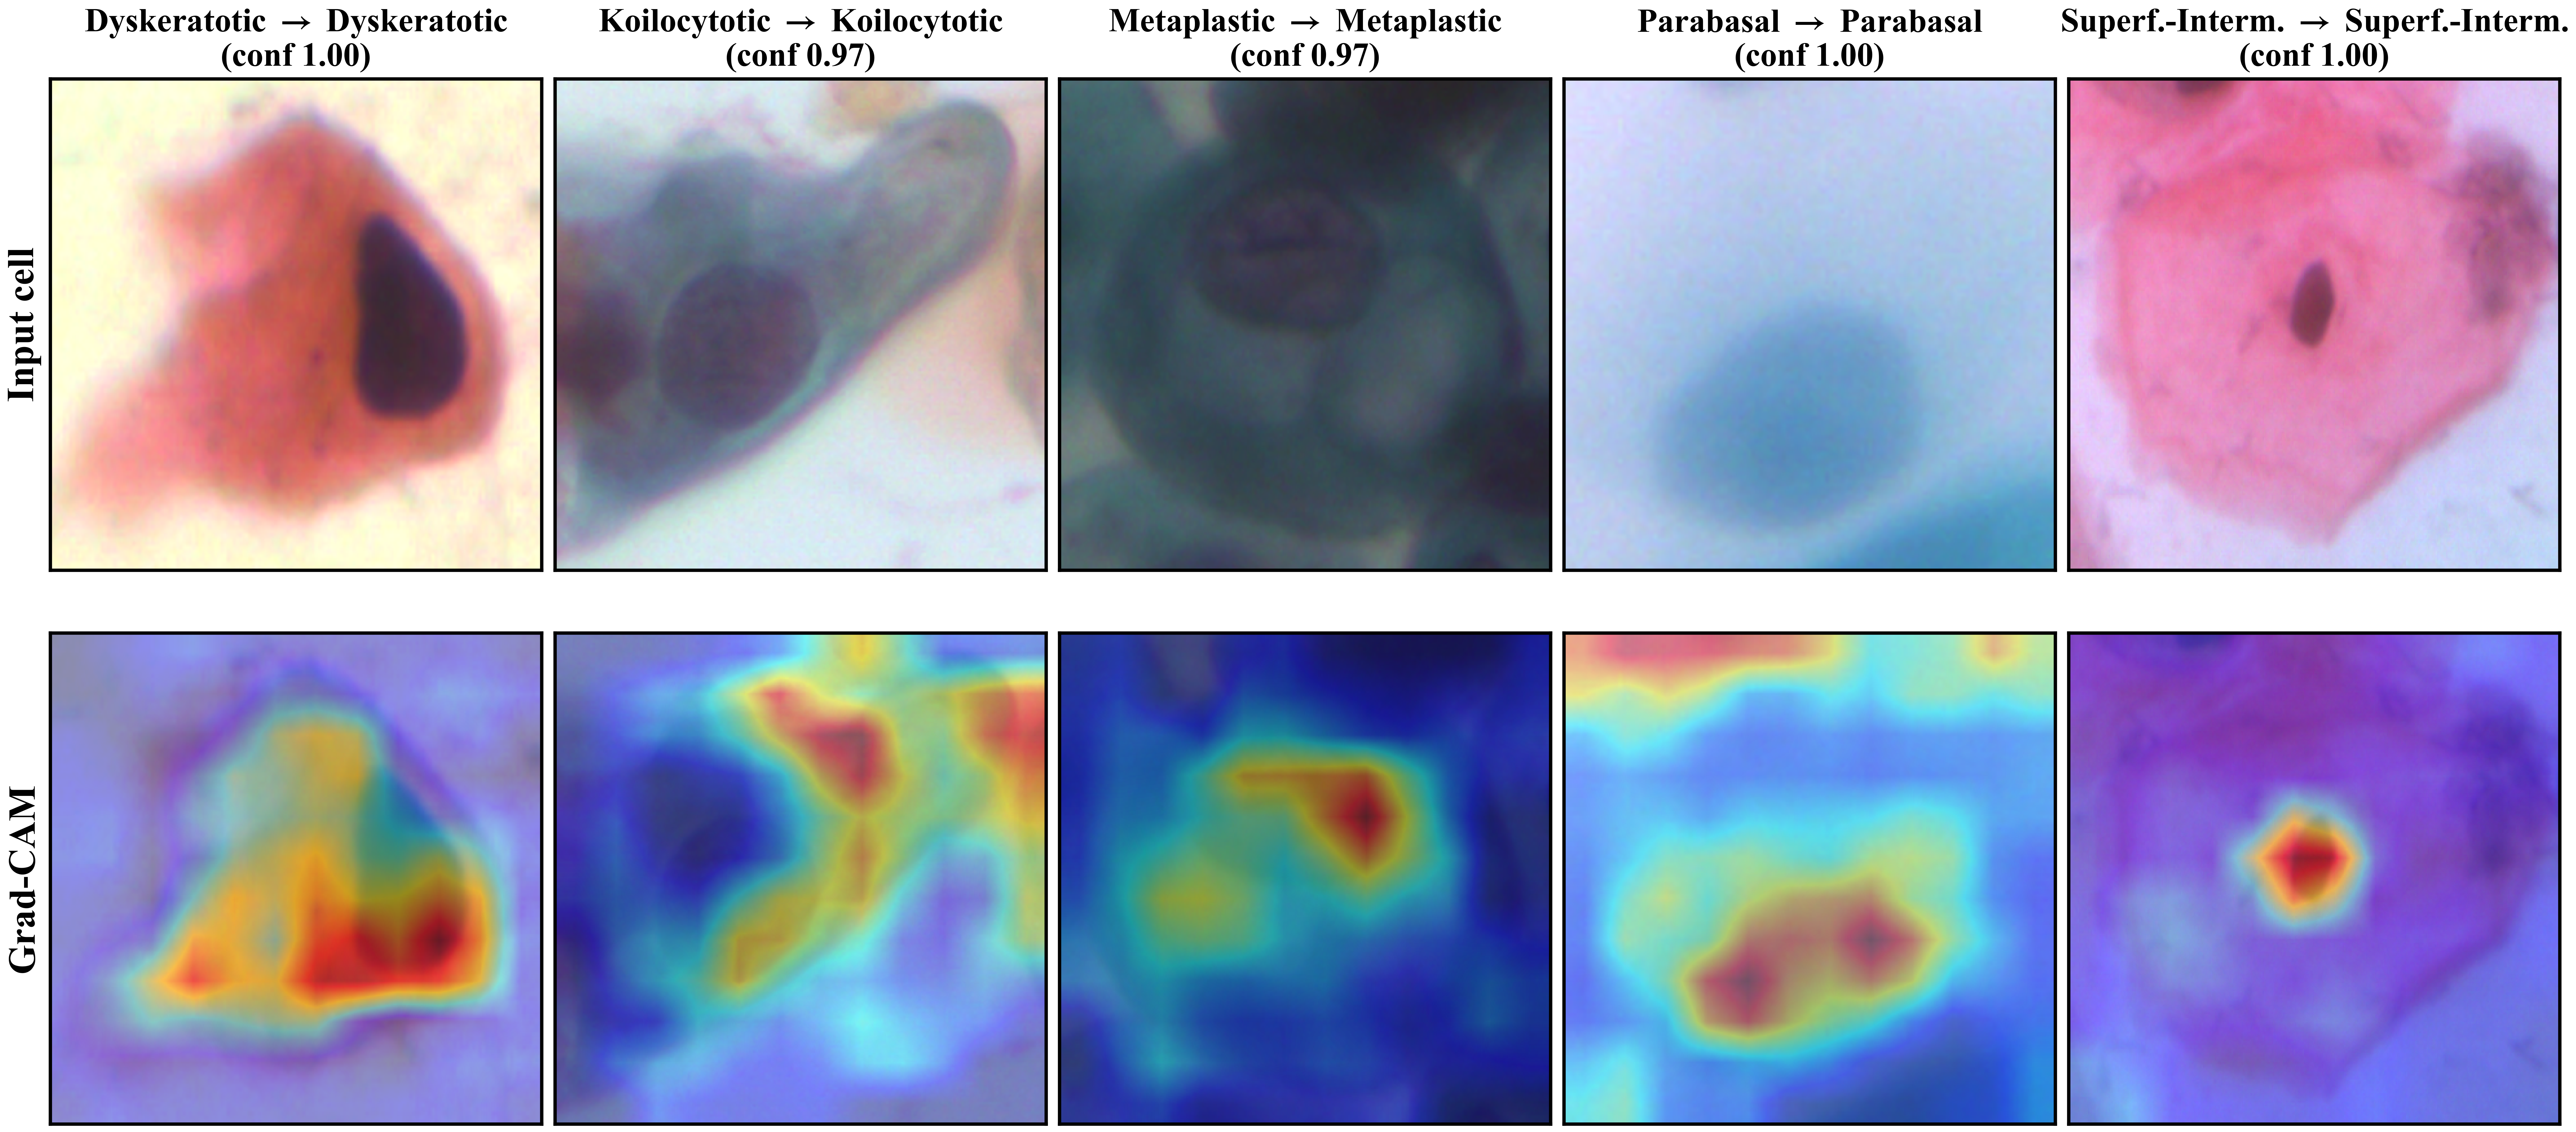
\includegraphics[width=\textwidth]{gradcam_student.png}
  \caption{\textbf{Grad-CAM attributions (student).} One representative cell per class: top row, input
  cell; bottom row, Grad-CAM overlay (true $\rightarrow$ predicted, confidence). Heatmaps localise to
  nuclear/cellular regions; all five sample cells are correctly classified at confidence
  $0.97\!-\!1.00$.}
  \label{fig:gradcam}
\end{figure*}
